\chapter{PDM之形变模拟}

\section{弹性模型}
\label{elasitcity_model}

在章节\ref{pdm_derivation}中,已经推导了近场动力学中关于线性材质的各向同性模型,其具体形式由式 \ref{eq:48}$\sim$\ref{eq:53} 所示。同时本文还给出了关于一般超弹性模型的推导框架,以应用于其他材质模型。考虑到线性模型的简单性,所以在本文工作中主要采用了这一模型。但从式 \ref{eq:48}$\sim$\ref{eq:53}给出的模型可以看出,其在理解上仍然不够具有物理直观,因此在本章节将对其进行重新表述,并给出本文工作超弹性模型的最终版本。

如前章节所述,在近场动力学中,由粒子 $j$ 施加给粒子 $i$ 的弹性内力密度可具体写为
\begin{equation}
\mathbf{T}\langle\mathbf{x}_j,\mathbf{x}_i\rangle = \frac{1}{2}A\frac{\mathbf{y}_j-\mathbf{y}_i}{|\mathbf{y}_j-\mathbf{y}_i|}
\end{equation}

其中 $\mathbf{x}$ 和 $\mathbf{y}$ 分别是粒子形变前和形变后的位置,力密度的方向即为粒子之间的连线方向,由$\frac{\mathbf{y}_j-\mathbf{y}_i}{|\mathbf{y}_j-\mathbf{y}_i|}$给定。$A$ 则代表力的大小,其包含所有的本构信息,并由式 \ref{eq:49} 给出(注意下标有所改变)

\begin{equation}
A = 4\omega_{ij}\left\{ad\frac{\mb{y}_j-\mb{y}_i}{|\mb{y}_j-\mb{y}_i|}\cdot\frac{\mb{x}_j-\mb{x}_i}{|\mb{x}_j-\mb{x}_i|}\theta_i
   +b\left(|\mb{y}_j - \mb{y}_i| - |\mb{x}_j - \mb{x}_i|\right) \right\}
\end{equation}

事实上,可以将其分解为各向均匀膨胀项(dilatational part)和剪切项(deviatoric part),从而更具有物理直观。为完成这一目标,首先需要将参数 $a$ 分解为两个部分:

\begin{equation}
a = a_1 + a_2 \qquad \mathrm{with}\quad a_1 = \frac{1}{2}\kappa ,\quad a_2 = -\frac{5\mu}{6}
\end{equation}

需要额外注意的是,当泊松比为 0.25 时,$a$ 等于0。在此情形下,膨胀度 $\theta_i$ 将消失,模型将回退到 bond based 情形,整个系统实际上也将退化为质点弹簧系统。不难看出 $\theta_i$ 的引入,是区分bond based 模型和 state based 模型的关键。将 $a$ 分解后,便可以将 $A$ 重新整理为

\begin{equation}
\begin{aligned}
A =4\omega_{ij}\left\{a_1d\frac{\mb{y}_j-\mb{y}_i}{|\mb{y}_j-\mb{y}_i|}\cdot\frac{\mb{x}_j-\mb{x}_i}{|\mb{x}_j-\mb{x}_i|}\theta_i
   +b\left(e_{ij} + \frac{a_2d}{b}\frac{\mb{y}_j-\mb{y}_i}{|\mb{y}_j-\mb{y}_i|}\cdot\frac{\mb{x}_j-\mb{x}_i}{|\mb{x}_j-\mb{x}_i|}\theta_i\right) \right\}
\end{aligned}
\end{equation}

其中$e_{ij} = |\mb{y}_j - \mb{y}_i| - |\mb{x}_j - \mb{x}_i|$为粒子之间的伸长量,其相当于连续介质力学中的柯西应变张量。注意在花括号中,第一项仅仅和体积模量 $\kappa$ 和膨胀度 $\theta_i$ 相关,而第二项仅仅和剪切模量 $\mu$ 相关。因此,上式已经成功将形变分解为膨胀项和剪切项两个部分。对于剪切项,可以进一步定义剪切伸长分量(deviatoric component of extension):

\begin{equation}
\begin{aligned}
e^d_{ij} \equiv& e_{ij} + \frac{a_2d}{b}\frac{\mb{y}_j-\mb{y}_i}{|\mb{y}_j-\mb{y}_i|}\cdot\frac{\mb{x}_j-\mb{x}_i}{|\mb{x}_j-\mb{x}_i|}\theta_i\\
                  =& e_{jk} - \frac{\delta}{4}\frac{\mb{y}_j-\mb{y}_i}{|\mb{y}_j-\mb{y}_i|}\cdot\frac{\mb{x}_j-\mb{x}_i}{|\mb{x}_j-\mb{x}_i|}\theta_i
\end{aligned}
\label{deviatoric_extension}
\end{equation}

从直观上看,$e^d_{ij}$相当于是移除总形变$e_{ij}$的各向均匀碰撞部分。经上述分解后,力密度大小 $A$ 可以最终写为

\begin{equation}
A = A_{dil} + A_{dev}
\end{equation}
其中 $A_{dil}$ 和 $A_{dev}$ 即分别为力密度大小的各向均匀膨胀部分以及剪切形变部分:
\begin{equation}
A_{dil}=4\omega_{ij}a\frac{\mathbf{y}_j-\mathbf{y}_i}{|\mathbf{y}_j-\mathbf{y}_i|}\cdot\frac{\mathbf{x}_j-\mathbf{x}_i}{|\mathbf{x}_j-\mathbf{x}_i|}\theta_i
\end{equation}

\begin{equation}
A_{dev}=4\omega_{ij}b(e_{ij}-\frac{\delta}{4}\frac{\mathbf{y}_j-\mathbf{y}_i}{|\mathbf{y}_j-\mathbf{y}_i|}\cdot\frac{\mathbf{x}_j-\mathbf{x}_i}{|\mathbf{x}_j-\mathbf{x}_i|}\theta_i)
       =4\omega_{ij}be^d_{ij}
\label{Adev}
\end{equation}

注意在上式中,动力学参数 $a$ 已经被重新定义。近场动力学的两个动力学参数 $a$,$b$ 的作用实际上相当于连续介质力学中的体积模量和剪切模量,甚至因为近场动力学由连续介质力学演变而来,这两个参数直接由体积模量及剪切模量表示:

\begin{equation}
a \equiv a_1d = \frac{9\kappa}{8\pi\delta^4} ,\qquad b = \frac{15\mu}{2\pi\delta^5},
\end{equation}

注意 $a$ 仅和 $\kappa$,而 $b$ 仅和 $\mu$ 相关。膨胀度 $\theta_i$ 、伸长比 $s_{ik}$(stretch)和权重函数仍然维持原有定义,具体写为

\begin{equation}
s_{ik}=\frac{|\mathbf{y}_k-\mathbf{y}_i|}{|\mathbf{x}_k-\mathbf{x}_i|} -1
\end{equation}

\begin{equation}
\omega_{ij} = \frac{\delta}{|\mathbf{x}_j-\mathbf{x}_i|}
\end{equation}

\begin{equation}
\theta_i = \frac{9}{4\pi\delta^4}\sum_{k=1}^N\omega_{ik}s_{ik}\frac{\mathbf{y}_k-\mathbf{y}_i}{|\mathbf{y}_k-\mathbf{y}_i|}\cdot(\mathbf{x}_k-\mathbf{x}_i)V_k
\end{equation}

$s_{ik}$ 衡量的是粒子间 bond 的伸长量。 $\omega_{ij}$ 为权重函数,其是单调递减的,即离中心粒子 $i$ 越近,则权重越大。注意 $\omega_{ij}$ 定义在材质空间(material space)而不是形变空间,因此其值取决于粒子的初始分布。最后,$\theta_i$ 衡量的是粒子 $i$ 所在位置的各向均匀膨胀度,其通过粒子 $i$ 的位置和其邻域范围内的其他粒子 $k$ 的位置来算得。仔细考虑可以发现,$\theta_i$ 的引入将使得粒子 $i$ 和粒子 $j$ 的相互作用力不仅仅和彼此相关,而是和粒子的整个邻域范围内的其他粒子相关。在使用基于显式欧拉积分的方法中(章节\ref{explicit_euler_method}),付出的代价仅仅是为每一个粒子,都计算其 $\theta_i$ 值,并不改变算法的复杂度。但对于隐式欧拉方法(章节\ref{implicit_euler_method}),情况则不同。因为刚度矩阵 $\textbf{K} = \frac{\partial \textbf{f}^{int}}{\partial \textbf{x}}$ 的计算同样需要考虑整个邻域,因而给整个算法的实现增加了一层复杂度,因此在较大规模仿真系统中,直接使用隐式欧拉积分以当前计算能力仍难具可行性。

\section{塑性模型}
塑性形变表示的是当材料的形变过大时,由于材料内部的屈服而导致无法回退到最开始的未形变状态,物质的内部结构被永久改变。
由于塑性行为的复杂性,现阶段关于近场动力学理论中塑性模型的研究仍然屈指可数。\mycite{Silling}{2007}在此工作中第一次提出了一个适用于近场动力学理论的塑性模型,这一模型在原理上类似经典理论中的 von Mises 流动模型。 Mitchell et al. 则根据这一模型,提出了一个关于近场动力学塑性行为的仿真框架\mycite{Mitchell}{2011}。但据本文所知,到目前为止,这一模型在学术界仅仅是停留在理论分析层面,而并没有相关工作对其进行验证。本文工作应为第一此在实际应用中使用这一模型,但针对图形学的应用特点做出了一些针对性的修改。

本文所用模型基于纯粹的剪切塑性流动理论(purely deviatoric plastic flow theory),因此我们需要将式\ref{deviatoric_extension}定义的剪切伸长量以加法形式分解为两部分:

\begin{equation}
e_{ij}^d = e_{ij}^e+e_{ij}^p
\end{equation}

其中 $e_{ij}^e$ 和 $e_{ij}^e$ 分别为剪切应变中剪切伸长量中的弹性部分和塑性部分。为将塑性模型集成进入原有的近场动力学弹性本构模型,我们需要将内力密度大小 $A$ 的剪切分量 $A_{dev}$(见式 \ref{Adev})重新定义为

\begin{equation}
A_{dev} = 4\omega_{ij}b(e_{ij}^d-e_{ij}^p)
\end{equation}

上式的目的在于在进行力计算时,将塑性形变部分从总的剪切形变部分中移除。对于弹性模型,则项 $e_{ij}^p$ 直接消失,上式回退到方程\ref{Adev}。$e_{ij}^p$ 是模拟塑性的最本质的部分,而塑性行为的仿真仿真需要两大关键步骤。第一是在仿真时物体形变的过程中,判断物体是否由弹性进入到塑性状态。第二则是根据形变的大小,更新总剪切形变中的塑性部分。

对于判断塑性是否发生,一般使用的是屈服方程 $f(A_{dev})$ (yield function)来进行决定:

\begin{equation}
f(A_{dev}) = \frac{(A_{dev})^2}{2}-\Psi_0,
\end{equation}

其中 $\Psi_0$ 代表进入塑性状态的阈值,值越大代表塑性愈难发生,而越小则代表物体很容易发生塑性形变。在上式中,如果$f(A_{dev})\leq 0$ 则处于弹性状态,而如果 $f(A_{dev}) > 0$,则意味着材料将发生塑性行为。

在塑性形变发生的情形下,需要重新计算物体所受的剪切力部分(膨胀项部分不受影响)。为此,我们需要将 $A_{dev}$ 屈服平面之上以获取真正的剪切力密度:

\begin{equation}
A_{dev}^c=\sqrt{2\Psi_0}\mathrm{sign}(A_{dev}),
\end{equation}

其中 $\mathrm{sign}(\cdot)$ 为符号方程。$A_{dev}^c$ 的值可进一步用于更新塑性形变部分 $e^p$ 的更新:

\begin{equation}
\triangle e_n^p = \frac{1}{2b}(A_{dev}-A_{dev}^c)
\end{equation}
\begin{equation}
e_{n+1}^p = (e_n^p+\triangle e_n^p)\mathrm{min}\big(1,\frac{\gamma}{|e_n^p+\triangle e_n^p|}\big).
\end{equation}

再上式中下标 $n$ 和 $n + 1$ 分别表示当前时间步和下一时间步。在时间步 $n$ 时,可以算得总的弹性形变量,当前塑性形变由前续仿真步累计而来,因此可以算得当前塑性形变部分的增量。注意,上式中的 $\gamma$ 参数用来对塑性的总量进行限制,这一参数并没有出现在\mycite{Mitchell}{2011}所提出的模型中,而是本文借鉴了\textcolor{blue}{(O'Brien et al. 2002)\parencite{OBrien2002}}所提出的加法模型,设计此参量。实验证明,在引入此参量之后,可以获得对于塑性行为更多的控制,以及对于仿真的稳定性也大有裨益。但值得注意的是,这一参数的引入并不符合真正的材料属性,即使在发生极大塑性形变行为下,材料也不可能重新进入弹性状态,因此 $\gamma$ 参数更多的是防止仿真过程中由于数值抖动而引起整个仿真崩溃。本文所用的塑性模型可总结为如图\ref{plasticity_model}所示:

\begin{figure}[!htb]
  \centering
  \captionsetup{justification=centering}
  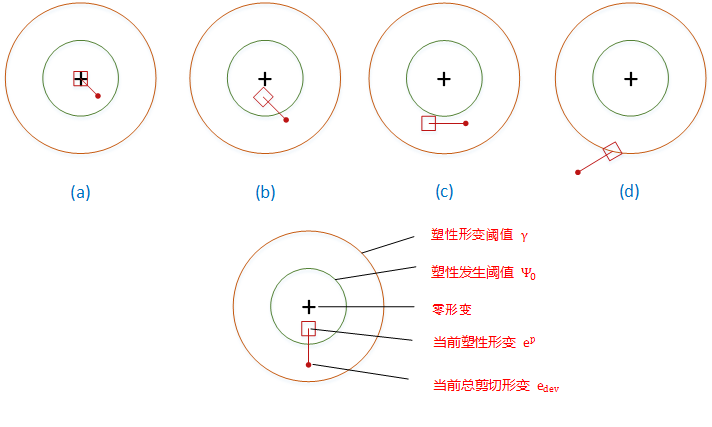
\includegraphics[width=\linewidth]{E:/Thesis-Master/chap/image/plasticity_model}

  \caption{\label{plasticity_model}
           塑性模型示意图。其中图(a)为弹性形变,图(c)和图(c)为塑性形变,图(d)表示超出塑性形变总量限制。
          }
\end{figure}


\section{离散化框架及嵌网格策略}
\label{discretization}

尽管基于粒子的无网格方法在物理计算上较为灵活方便,但付出的代价就是需要重新产生网格来进行表示。不同于工程领域只关注于计算的准确性,图形学领域中的应用实际上更关注视觉效果,所以炫酷的视觉渲染输出尤为重要。纯粹使用基于粒子的方法来进行渲染在流体仿真中较为常见,例如可以使用基于屏幕空间(Screen-based)的渲染技术来取得不错的效果。但现有应用的视觉输出都是大部分采用基于网格(mesh)的渲染达到的,甚至对于高质量的流体渲染,通常的方式也是离线将粒子云使用相关算法来重建网格,如Marching Cube等。但重建网格的方式对于固体仿真尤其是碎裂仿真几乎是不可能,因为纯粹基于粒子位置信息很难对裂纹进行重建和表达。因此,更常见的方式是采用嵌网格的办法来对物体的形变和碎裂进行显示追踪,本文工作亦使用这种方式。

使用嵌网格方法的优点是网格的边界即代表物体的表面,因此在渲染时能够提供更多的细节,并且也比较容易反映仿真过程中物体的形变以及碎裂。在本文工作中,我们直接使用四面体网格来离散整个仿真物体,并且将仿真粒子置于四面体的几何中心,亦即每一个四面体即代表一个仿真粒子,如图\ref{embedded_mesh}所示。

\begin{figure}[!htb]
  \centering
  \captionsetup{justification=centering}
  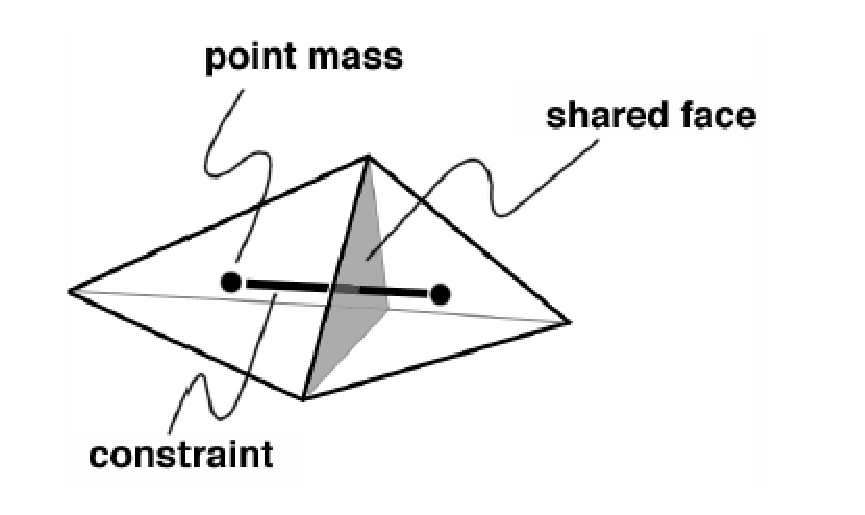
\includegraphics[width=0.6\linewidth]{E:/Thesis-Master/chap/image/embedded_mesh}

  \caption{\label{embedded_mesh}
           离散化框架与嵌网格。本文工作将仿真粒子置于四面体的中心,相邻的粒子共享一个四面体表面,并且粒子之间通过 bond 相连。
          }
\end{figure}

在将仿真粒子置于网格单元体的中心后,便可以根据设定的邻域半径 $\delta$ 来对每一个粒子的邻域 $H_\mb{x}$(family)进行初始化。对于搜寻邻域范围内的粒子,比较 naive 的方式是直接双重循环遍历,计算粒子对之间距离,然后判断是否位于其邻域范围内,如此整个算法的复杂度为 $O(N^2)$。 但更具效率的方式是进行空间哈希,将粒子先置于均匀分布的空间栅格(grid)中,然后针对每一个 grid,只需要搜寻其周围 27 个直接相邻的栅格中粒子,然后判断是否位于邻域半径 $\delta$ 内,这一算法几乎是 $O(N)$ 的,从而能大幅度提高粒子搜寻的效率。不过,粒子的邻域初始化是仿真开始之前的预处理阶段,对于包含四面体数较少的物体,使用 $O(N^2)$ 并不影响整体仿真效率。

在物体发生形变之后,需要对于拓扑网格进行更新,即需要改变四面体网格中顶点的位置。本文工作所采用的方法是基于连接该顶点的四面体中的仿真粒子位置,以加权平均的方式来进行更新,具体而言:

\begin{eqnarray}
\omega_{\mathrm{v}} &=& \sum_{\mathrm{p}} \frac{1}{4}m_{\mathrm{p}}\\
\textbf{v}_{\mathrm{v}} &=& \frac{1}{\omega_{\mathrm{v}}}\sum_{\mathrm{p}}\frac{1}{4}m_{\mathrm{p}}\textbf{v}_{\mathrm{p}}\\
\mathbf{x}_{\mathrm{v}}^{t+1} &=& \mathbf{x}_{\mathrm{v}}^{t} + \Delta t\textbf{v}_{\mathrm{v}}
\end{eqnarray}

其中下标 $\mathrm{p}$ 和 $\mathrm{v}$ 分别表示粒子(particle)和网格顶点(vertex),$m_{\mathrm{p}}$ 和 $\textbf{v}_{\mathrm{p}}$ 分别是粒子的质量和速度,$\textbf{v}_{\mathrm{v}}$ 和 $\textbf{x}_{\mathrm{v}}$分别是网格顶点的速度和位置。在具体实现时,并不需要逐顶点来进行更新,因为一般不针对每一顶点存储与其相连的四面体,而可以直接通过遍历四面体,然后将四面体的四个顶点的权值和速度分别累加,累加完所有权值和速度之后,再将累加的速度除以权值即可。

值得注意的是,如果仅针对形变体问题,将仿真粒子置于四面体中心其实并不直观,并且随着仿真的进行,仿真粒子并不完全位于四面体的中心,而是会有所偏离。虽然在本文工作的实验中,并未发现明显的异常情况,但实际上在极大形变下,这一缺陷可能会体现出来。更为简单的方式是直接令仿真粒子对应到四面体的顶点上,这样粒子位置即顶点位置,处理起来更为方便。本文工作采用此种离散方式的理由是为了方便后续的碎裂引起的拓扑网格更新,其不仅仅是改变顶点的位置,还需要直接改变网格的拓扑结构,因为近场动力学的碎裂实质上是 bond 的消除,如果将仿真粒子对应到顶点则很难在四面体网格上进行体现,详见章节xxx。



\section{实验结果}
\label{deformation_results}

本文工作所有实验(包括碎裂仿真实验,章节\ref{fracture_results})都运行于一台 CPU 配置为 3.5GHz, Intel Core i7-5930,内存为 32GB 的主机。实验所用的物体模型由开源软件 TetGen 生成\mycite{Si}{2015},其可以直接通过给定粒子云或者给定 .Obj 格式的表面网格来产生高质量四面体网格。而最终的渲染输出,都是直接从四面体网格中提取表面网格,使用 POV-Ray \footnote{http:www.povray.org/} 开源光线追踪软件并配置相关光照参数渲染而成。

本文工作所有实现基于前述章节所述的近场动力学弹塑性模型,以及后续章节将要阐述的碎裂和各向异性模型,并且使用 openMP 来进行多线程实现。本章节将主要阐述基于 PDM 方法产生形变仿真效果。

为确保所用本构模型的正确性,本文实通过多样化材质的属性参数分别进行仿真实验,并和 FEM 方法进行了充分的对比。
其中图\ref{demo_pull_armadillo} 为 Armadillo 的各向同性线性形变实验。初始时 Armadillo 四肢被固定,并且其背部拉扯到一定位置,松开后 Armadillo 便往前形变。可以看到即使 Armadillo 四肢被过度拉伸,但并没有产生明显的数值塑性,整个形变过程非常自然。


\begin{figure}[!htb]
  \centering
  \captionsetup{justification=centering}
  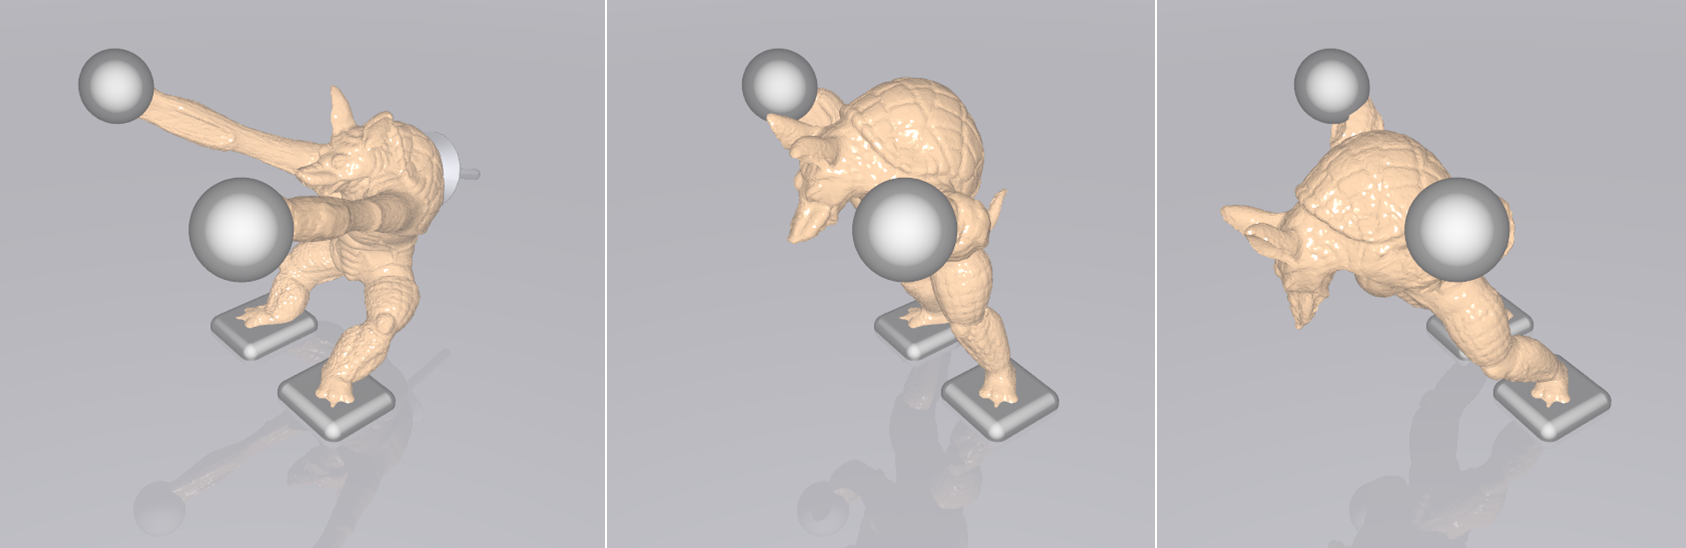
\includegraphics[width=0.9\linewidth]{E:/Thesis-Master/chap/image/demo_pull_armadillo}

  \caption{\label{demo_pull_armadillo}
           Armadillo 各向同性线性形变实验。初始时 Armadillo 四肢被固定,并且其背部拉扯到一定位置,然后松开。
          }
\end{figure}

在图\ref{demo_impact_upside}实验中,本文比较了物体的弹性形变和塑性形变。不同材质的物质被以恒定速度运行球从上沿方向撞击。其中弹性物体被撞击后发生形变,但能恢复到初始状态。塑性物体被撞击后会发生塑性形变,并不能恢复到原始位置。

\begin{figure}[!htb]
  \centering
  \captionsetup{justification=centering}
  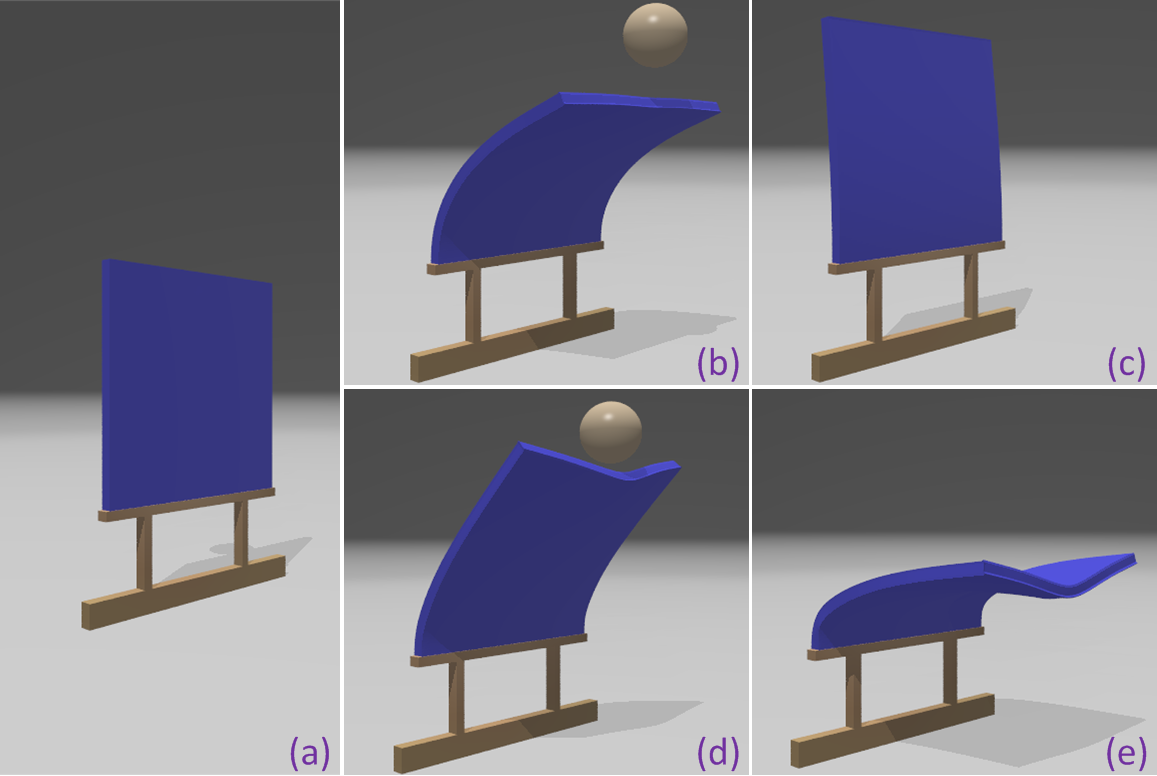
\includegraphics[width=0.7\linewidth]{E:/Thesis-Master/chap/image/demo_impact_upside}

  \caption{\label{demo_impact_upside}
           弹性形变和塑性形变对比实验。不同材质的物质被以恒定速度运行球从上沿方向撞击。图(a)表示相同的初始状态。图(c)表示弹性物体被撞击,然后发生形变,但是在图(c)中,形变被恢复。图(d)表示物体被撞击后发生塑性形变,并且如图(e)所示,并不能恢复到原始位置。
          }
\end{figure}

图\ref{compare_different_poisson_ratio}表示对于弹性材料(伸长的beam)不同泊松比的对比实验。在 bond based 模型中,泊松比被固定为 0.25,如\mycite{Levine}{2014}。使用基于 state based的模型能够破除这一限制,在材质属性的表达能力上达到同连续介质理论同等的水平。

\begin{figure}[!htb]
  \centering
  \captionsetup{justification=centering}
  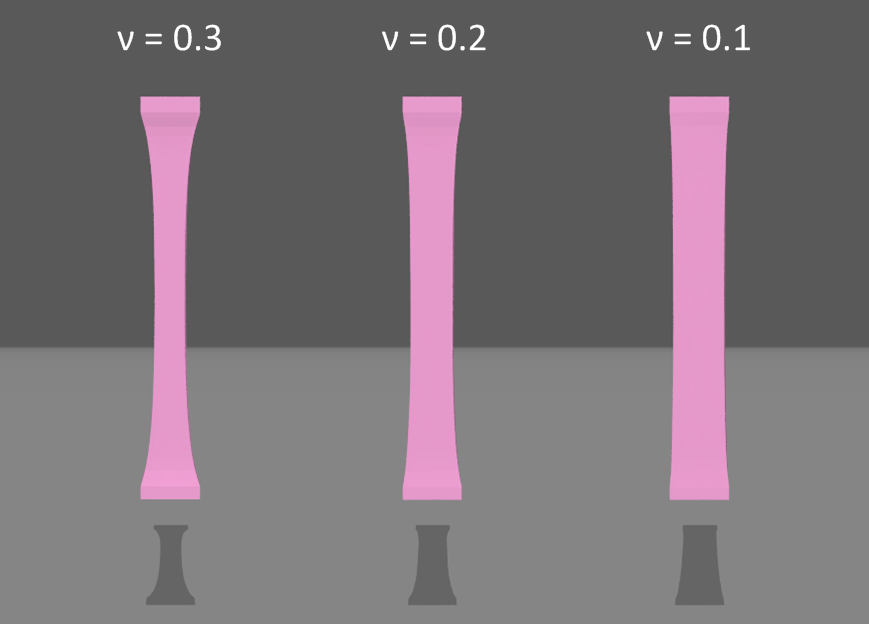
\includegraphics[width=0.7\linewidth]{E:/Thesis-Master/chap/image/compare_different_poisson_ratio}

  \caption{\label{compare_different_poisson_ratio}
           不同泊松比对比实验。泊松比越大,则不可压性质越明显。
          }
\end{figure}

最后,本文进行了四组同 FEM 的对比实验。其中\ref{demo_strip_vs_fem}为长条在重力下的弯曲实验。可以看到,近场动力学方法和 FEM 方法取得了几乎一致的效果。

\begin{figure}[!htb]
  \centering
  \captionsetup{justification=centering}
  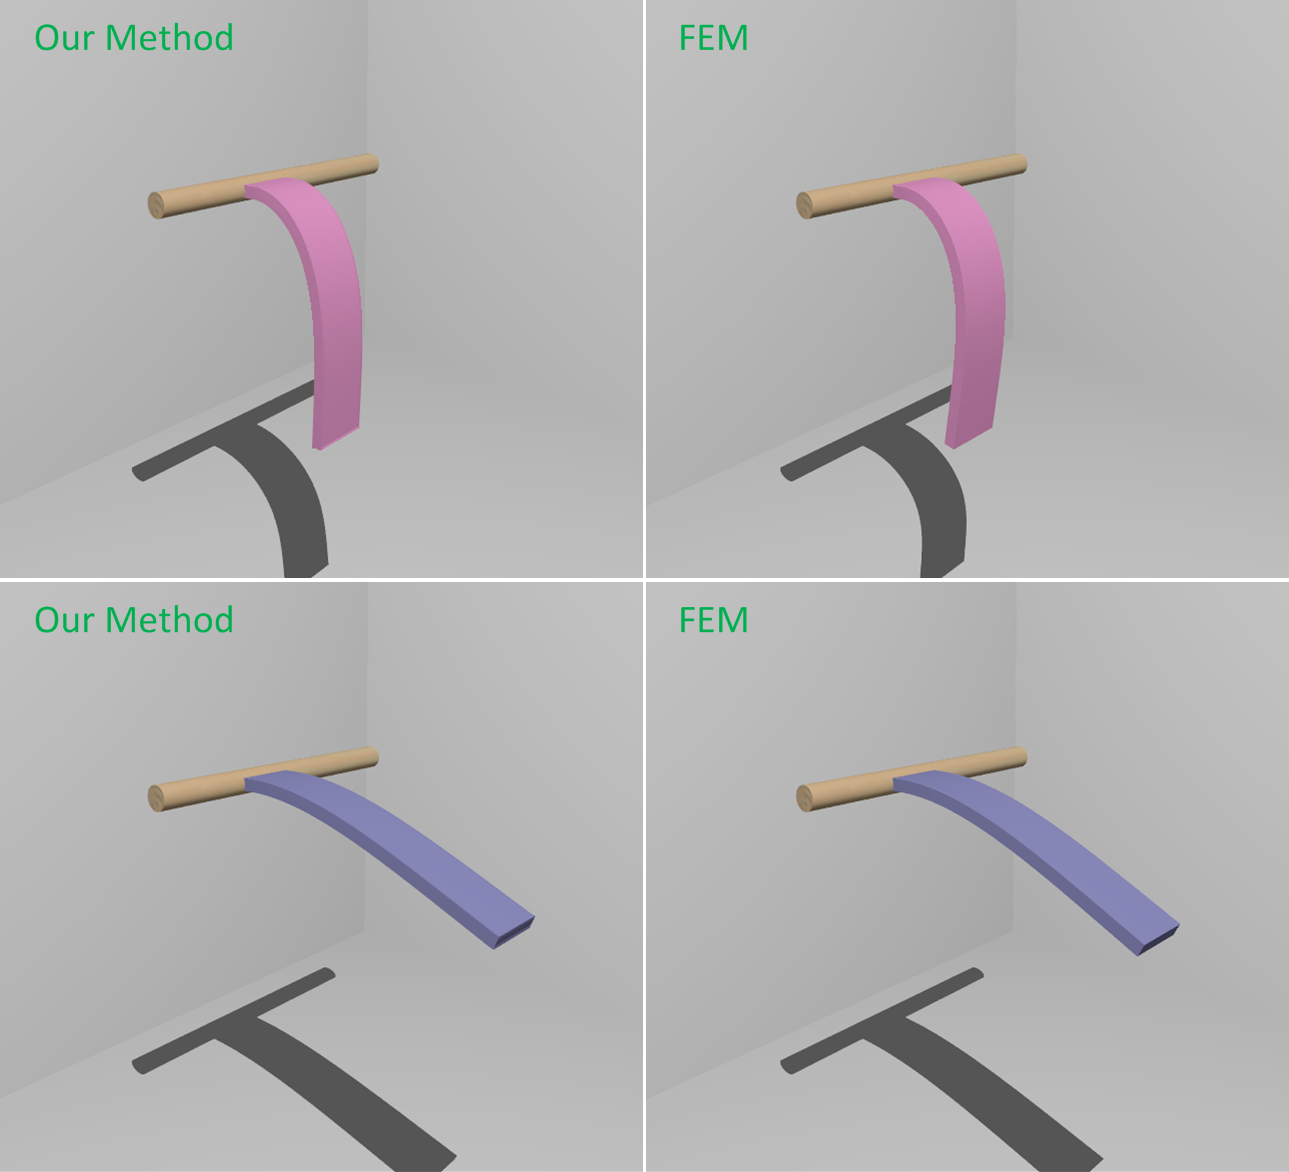
\includegraphics[width=0.7\linewidth]{E:/Thesis-Master/chap/image/demo_strip_vs_fem}

  \caption{\label{demo_strip_vs_fem}
           不同硬度的长条弯曲实验。左边为本文方法所取得的效果,右图为 FEM 方法效果。可以看到,两者取得了几乎一致的效果。
          }
\end{figure}

图\ref{demo_bar_oscillate_vs_fem}所示实验为晃动的 Bar。仿真初始时, Bar 被摆到一定角度位置,然后松开。对于这种大形变行为,可以显著感受到使用线性弹性模型的 FEM 方法将出现明显的不自然行为。并且可以看出,本文所提的线性近场动力学模型和 FEM 中的共旋线性模型在效果上几乎完全一致。本文进一步对两者的误差进行衡量,发现两者位置偏离小于 10\%。位置偏移通过 $Error = \frac{|\bm{x}_p-\bm{x}_p^{ref}|}{d}$,其中 $d$ 为物体包围盒的对角长度。

\begin{figure}[!htb]
  \centering
  \captionsetup{justification=centering}
  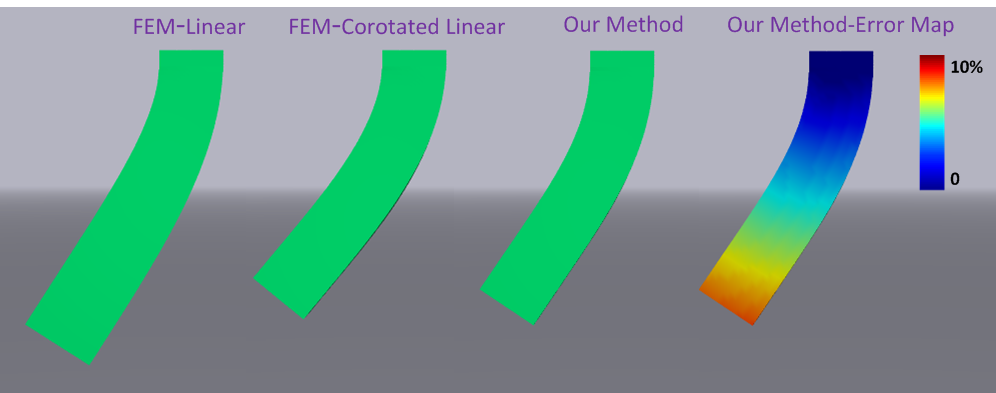
\includegraphics[width=0.9\linewidth]{E:/Thesis-Master/chap/image/demo_bar_oscillate_vs_fem}

  \caption{\label{demo_bar_oscillate_vs_fem}
           Bar 晃动实验。最左图为 FEM 线性模型,可以看到明显的不自然现象。中间两图分别为共旋线性模型和近场动力学方法,两者效果几乎完全一致。右图为误差图,基本上小于 10\%。
          }
\end{figure}

从效果上看,近场动力学中的线性模型要远好于 FEM 中的线性模型,并且可以取得和 FEM 中的共旋线性模型相比的效果。原因在于并没有使用 FEM 中柯西应变张量,因此并不是几何线性中。进一步而言,在近场动力学中,纯粹的刚性变化并不会像 FEM 中的线性模型一样,产生虚拟的力(ghost force),从而大幅度拓展近场动力学模型的适用范围。在图\ref{demo_bar_twist_vs_fem}中,本文还对扭曲的 Bar 进行对比实验,从图中可以更明显的看出 FEM 线性模型的缺陷。图\ref{demo_armadillo_vs_fem}展示为 Armadillo 复杂的周期性振荡形变行为,可以看到,在如此复杂的形变行为上,近场动力学仍然取得了和 FEM 非常一致的效果。

\begin{figure}[!htb]
  \centering
  \captionsetup{justification=centering}
  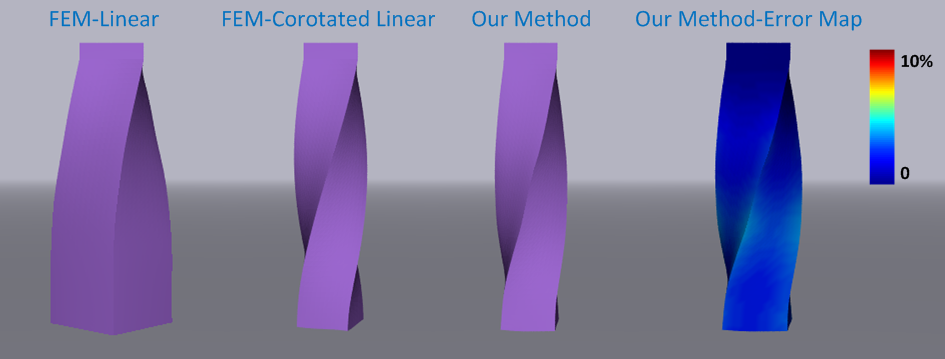
\includegraphics[width=0.9\linewidth]{E:/Thesis-Master/chap/image/demo_bar_twist_vs_fem}

  \caption{\label{demo_bar_twist_vs_fem}
           Bar 扭曲实验。最左图为 FEM 线性模型,可以看到更为明显的不自然现象。中间两图分别为共旋线性模型和近场动力学方法,两者效果几乎完全一致。右图为误差图,基本上小于 10\%。
          }
\end{figure}

\begin{figure}[!htb]
  \centering
  \captionsetup{justification=centering}
  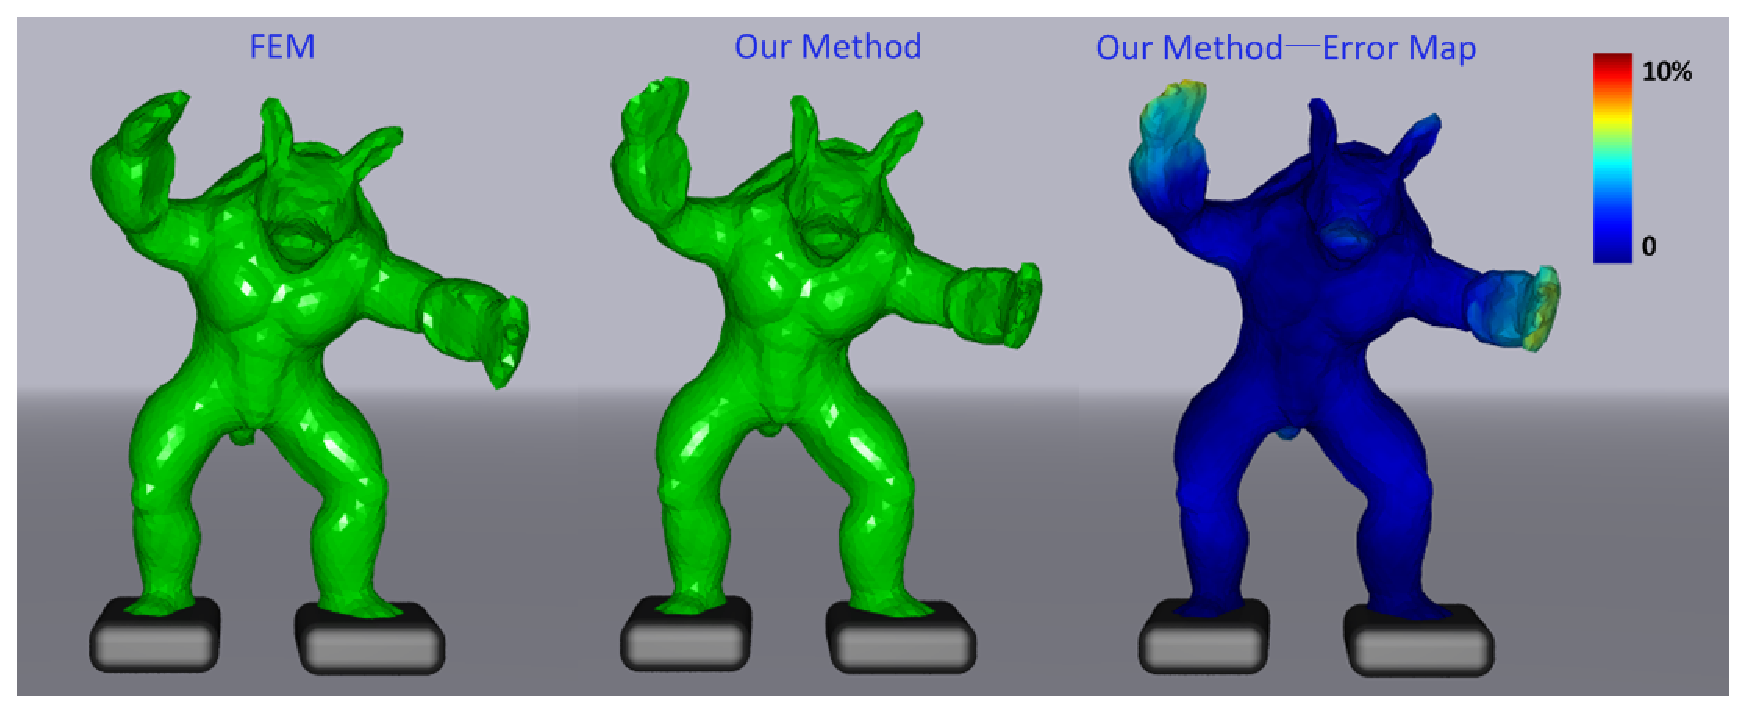
\includegraphics[width=0.9\linewidth]{E:/Thesis-Master/chap/image/demo_armadillo_vs_fem}

  \caption{\label{demo_armadillo_vs_fem}
           Armadillo 周期性振荡实验。左图为 FEM 方法,中图为近场动力学方法,右图为误差图。即使对于这种复杂的周期性振荡形变行为,两者仍然取得了非常一致的效果。
          }
\end{figure}

下表\ref{deformation_results_table}展示了上述形变仿真实验所有模型参数以及物理参数。。从表中所示数据来看,近场动力学方法能够取得和 FEM 类似的计算效率,但近场动力学方法更易实现以及并行化。

\begin{table*}[htb]
\centerline{
\resizebox{1.3\textwidth}{!}{
\begin{tabular}{lccccccccccccc}
  \hline
  \hline
  Examples & particle num & $\delta$ & bond num & $\kappa$ & $\mu$ & $\rho$            & $\Psi_0$ & $\frac{\gamma}{|\mathbf{x}_j-\mathbf{x}_i|}$ & $s^w_{(k)(j)}$ & $\Delta t$ &$\lambda_a$    & $\lambda_l$  & performance\\
           &              &          &          &   (KPa)   & (KPa)  &(Kg/$\mathrm{m}^3)$&          &                                              &                & (s)       &   &   &(s/step)\\
  \hline
  Armadillo [Figure~\ref{demo_pull_armadillo}]           & $4.2\times10^5$ & 1.50$\lambda$ & $7.5\times10^7$ & $6.3\times10^4$   & $3.8\times10^4$          & 1000 & $\infty $ & 0.0             & $\infty$ & $1.0\times10^{-4}$          &$0.002$&0.001& $\sim5.3$ \\
  Elastic Wall [Figure~\ref{demo_impact_upside}(b)(c)]  & $3.0\times10^5$ & 1.45$\lambda$ & $5.0\times10^7$ & $1.0\times10^{4}$ & $6.0\times10^{3}$        & 1200 & $\infty $ & 0.0             &$\infty$  & $5.0\times10^{-5}$   &0&0& $\sim2.4$ \\
  Plastic Wall [Figure~\ref{demo_impact_upside}(d)(e)]  & $3.0\times10^5$ & 1.45$\lambda$ & $5.0\times10^7$ & $1.0\times10^{4}$ & $6.0\times10^{3}$        & 1200 & $10^{26}$ & 0.2             & $\infty$ & $5.0\times10^{-5}$   &0.0005&0& $\sim2.4$ \\
  Beam Stretch [Figure~\ref{compare_different_poisson_ratio}]        & $2.2\times10^4$ & 1.0 $\lambda$ & $1.3\times10^6$ & $2.0\times10^3$   & $(9.2,1.5,2.2)\times10^2$& 1000 & $\infty$  & 0.0             &$\infty$  & $1.0\times10^{-5}$ &0&0& $\sim0.2$ \\
  Soft Beam Bend [Figure~\ref{demo_strip_vs_fem}]      & $4.5\times10^4$ & 1.0 $\lambda$ & $6.9\times10^6$ & $6.3\times10^3$   & $3.8\times10^3$          & 1000 & $\infty $ & 0.0             & $\infty$ & $5.0\times10^{-5}$   &0&0& $\sim0.6$ \\
  Stiff Beam Bend [Figure~\ref{demo_strip_vs_fem}]     & $4.5\times10^4$ & 1.0 $\lambda$ & $6.9\times10^6$ & $3.3\times10^4$   & $2.0\times10^4$          & 1000 & $\infty $ & 0.0             & $\infty$ & $2.5\times10^{-5}$ &0&0& $\sim0.6$ \\
  Bar Swing [Figure~\ref{demo_bar_oscillate_vs_fem}]     & $9.2\times10^3$ & 1.11 $\lambda$ & $1.5\times10^5$ & $5.0\times10^3$   & $5.0\times10^3$          & 1000 & $\infty $ & 0.0             & $\infty$ & $1.0\times10^{-4}$ &0&0& $\sim0.05$ \\
  Bar Twist [Figure~\ref{demo_bar_twist_vs_fem}]     & $9.2\times10^3$ & 1.34 $\lambda$ & $1.5\times10^5$ & $1.0\times10^3$   & $6.0\times10^2$          & 1000 & $\infty $ & 0.0             & $\infty$ & $1.0\times10^{-4}$ &0&0& $\sim0.06$ \\
  Armadillo Vibrate [Figure~\ref{demo_armadillo_vs_fem}]     & $2.0\times10^4$ & 1.38 $\lambda$ & $1.8\times10^6$ & $5.0\times10^3$   & $3.0\times10^3$          & 1000 & $\infty $ & 0.0             & $\infty$ & $5.0\times10^{-4}$ &0&0& $\sim0.2$ \\
  \hline
\end{tabular}
}
}
\caption{形变仿真中的模型参数、仿真参数、及效率数据。其中 $\lambda$ 是四面体网格的平均边长度,用于邻域的初始化。}
\label{deformation_results_table}
\end{table*}

\section{本章小结}
本章主要研究基于近场动力学方法的弹塑性形变模拟。本章最开始给出了关于近场动力学弹性模型的一个更具物理直观的重新表述,其将力密度 $A$ 分解为各向均匀膨胀部分以及剪切部分。然后基于经典理论中的 von Mises 流动模型,本章还给出了适用于近场动力学理论中的塑性本构模型。接着详细介绍了本文所用的离散框架以及嵌网格策略,并且给出在物体形变时,更新网格顶点位置的方法。最后本章还展示了使用所提近场动力学弹塑性模型取得的逼真视觉效果,并和 FEM 方法进行了充分对比。可以看到,本文所提方法能够准确的对材质的属性进行表达,在效果能够取得和 FEM 共旋线性模型相当的效果,而要远好于 FEM 线性模型。